\documentclass[acmtog]{acmart}
\usepackage{graphicx}
\usepackage{subfigure}
% Title portion
\title{Assignment 2 : Create A B-spline Surface} 
\author{Name:\quad yongjiawei  \\ student number:\quad 2019533095
	\\email:\quad yongjw@shanghaitech.edu.cn}

% Document starts
\begin{document}
\maketitle

\vspace*{2 ex}


\section{Introduction}
In the last assignment, we create our first graphics program using OpenGL, which loads mesh from object file, and we implement a camare that can move in the space and phone shading model.
\\\\ In this assignment, we need to create our first B-spline curve with an iterative evaluation algorithm and render the surface mesh.
\\\\The main work I implemented is to use de Boor algorithm to consruct a B-spline surface, render the B-spline surface in OpenGL, based on the B-spline, construct a Non-Uniform Rational B-Spline (NURBS) surface,texture the B-Spline surface,Implement the UI function that enables moving control points to change the surface mesh.\label{key}

\section{Implementation Details}
\subsection{Use de Boor algorithm to construct a B-Spline surface }
In this part, we need to realize de Boor algorithm, first generate a MeshSur ,initialize all the paramter, the call function initalize to generate all the point of the given samplestep. The concrete process is to use de Boor algorithm.
\subsection{Render B-Spline surface with VAO, VBO in OpenGL}
After the construction of B-spline surface, we already get the point data of the surface include the position, normal and texture. Then we can easily create the VBO that bind the data of the surface, then we can bind relative index of each point to draw in triangle mode or in line mode.


\begin{figure}[h]
	\centering
	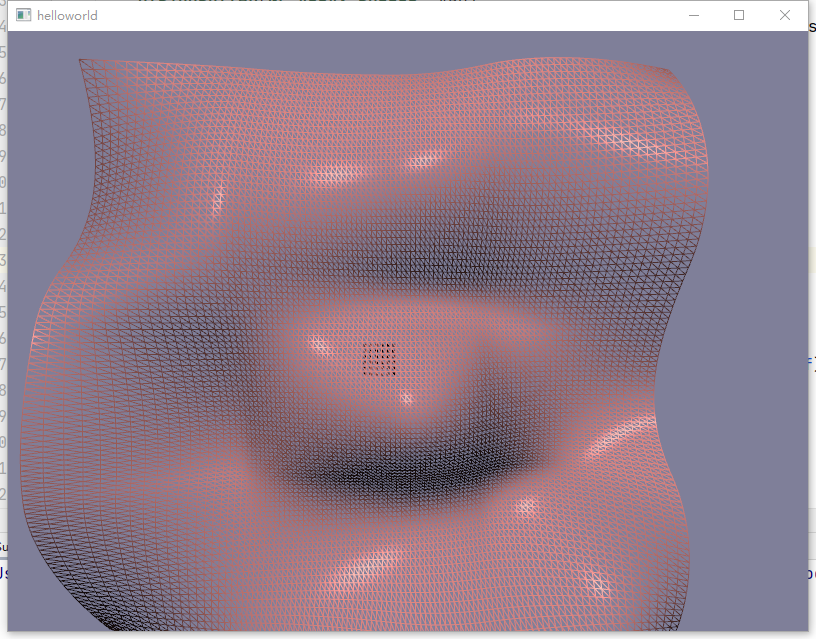
\includegraphics[width=8cm,height=6cm]{gl triangle mode.png}
	\caption{gl triangle mode.png .}
\end{figure}

\begin{figure}[h]
	\centering
	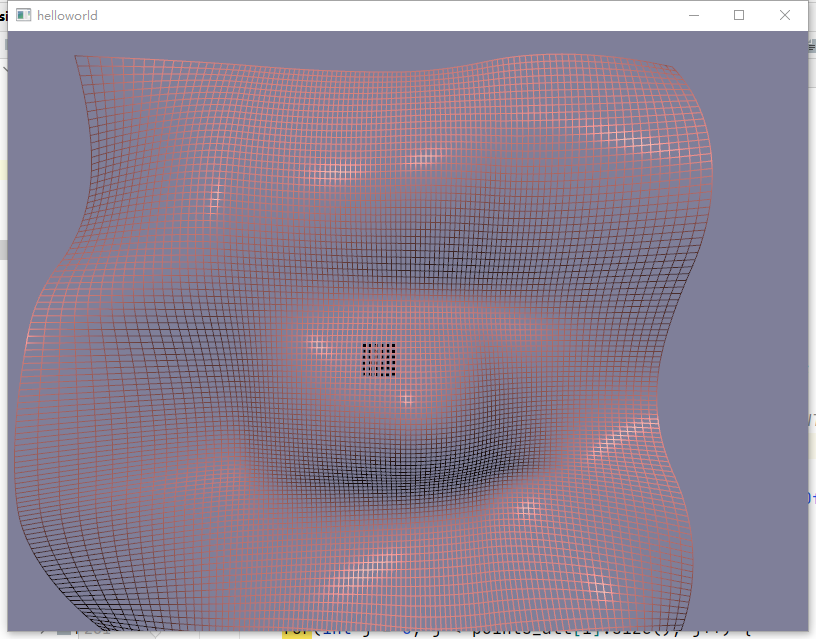
\includegraphics[width=8cm,height=6cm]{gl line mode.png}
	\caption{gl line mode.png .}
\end{figure}

\subsection{Based on the B-spline surface evaluation, construct a Non-Uniform Rational B-Spline (NURBS) surface}
A Non-Uniform Rational B-Spline(NURBS) surface is the general case of B-Spline surface, in NURBS, each controlpoint takes a weight, which is connected to the influence of the control point. So I create a new class nurBsplineSurface ,the difference between the two class is that in the new class, a glm::vec4 is passed to the DeBoorCurve function, then pass out a glm::vec4 , then we can calculate the final coordinate of each point.Modify the weight of one controlpoint, only part of the surface changed.

\begin{figure}[h]
	\centering
	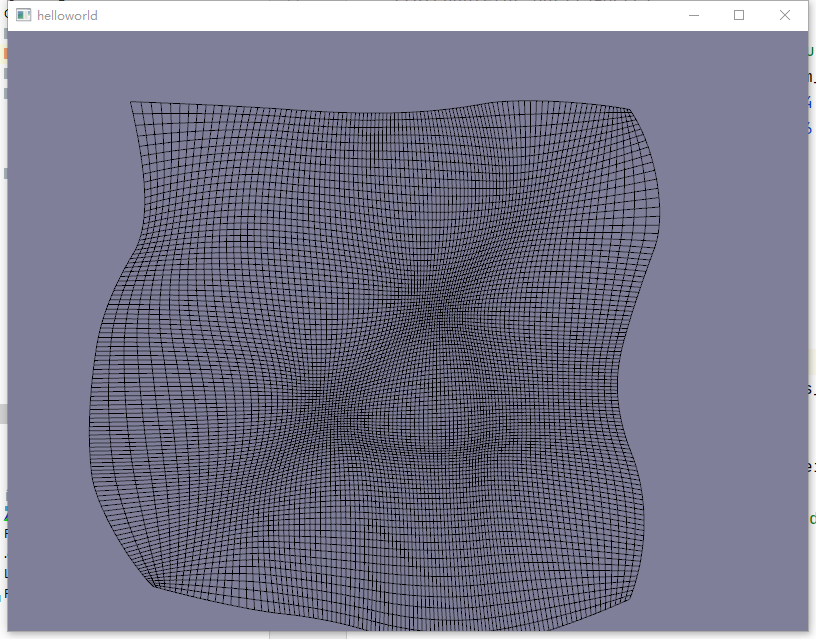
\includegraphics[width=8cm,height=6cm]{weight1.png}
	\caption{weight1.png .}
\end{figure}
\begin{figure}[h]
	\centering
	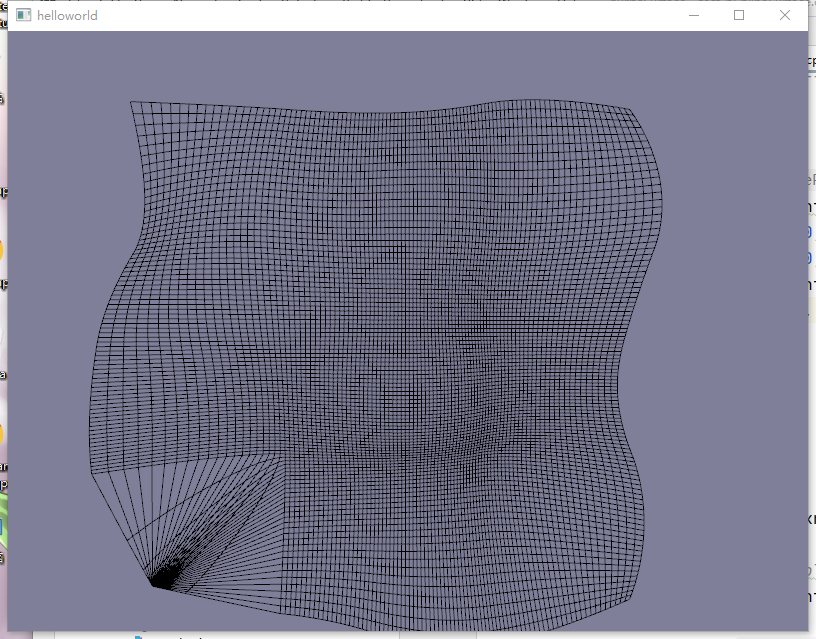
\includegraphics[width=8cm,height=6cm]{weight2.png}
	\caption{weight2.png .}
\end{figure}

\subsection{Texture the B-Spline surface }
In this part, we need to texture the surface. First we need to load and create texture, relative method is sample. then we need to apply the texture. At version 1, I simply adapt the texture coordinate on average, as Fig.5, the distortion of which is obvious. At version2, I adapt the texture coordinate by the ratio of this point relative to its same line index and same column index ,mapping the ratio to the texture, as Fig 6,
the distortion is decreased.
\begin{figure}[h]
	\centering
	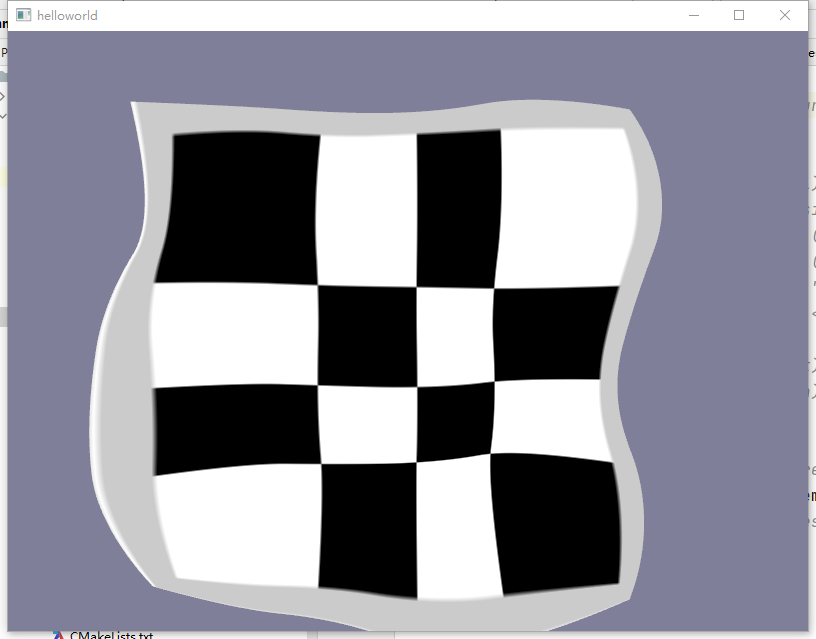
\includegraphics[width=8cm,height=6cm]{texture v1.png}
	\caption{texture v1.png .}
	
		\centering
	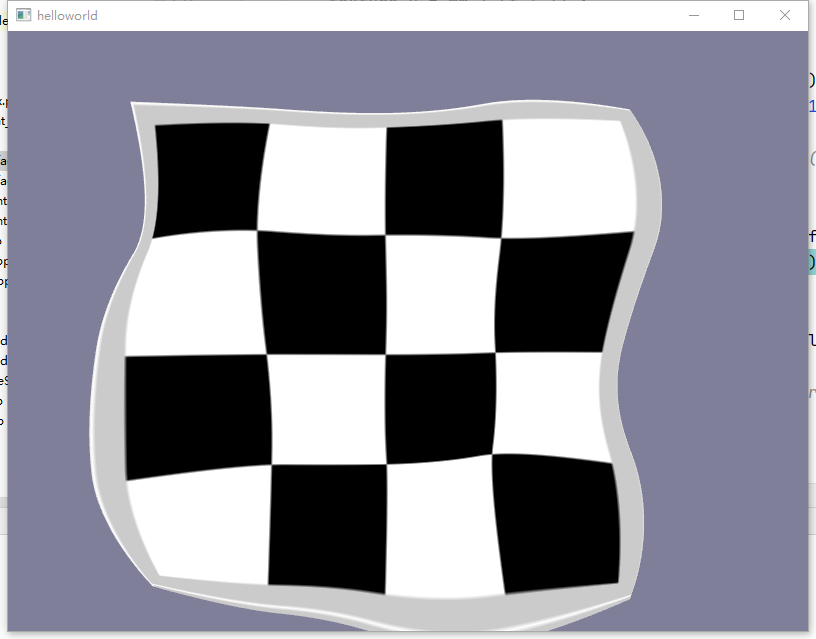
\includegraphics[width=8cm,height=6cm]{texture v2.png}
	\caption{texture v2.png .}
\end{figure}

\begin{figure}[h]

\end{figure}

\subsection{Implement the UI function that enables  moving control points to change the surface mesh}
In this part, main work is to use mouse to darg the controlpoint, then modify the shape of the final surface.
After one click of left botton, I get the position of curse, then calculate the nearest point and make sure the distance is less than a given value, if so, the position of that selected point will be modified by the change of curse.

\begin{figure}[h]
	\centering
	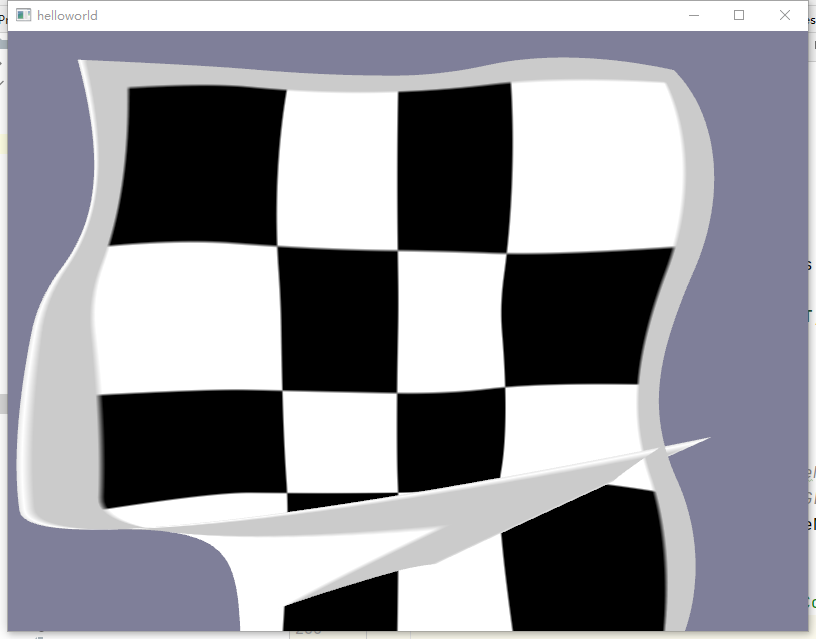
\includegraphics[width=8cm,height=6cm]{change point.png}
	\caption{change point.png .}
\end{figure}

\section{Results}
B-Spline curve is a better way to generate a curve than Bezier curve because B-spline is kind of partly, once you modify one single point, you can just change part of the origin feature. NURBS is a more general case, the influence of each controlpoints can be modified. By using these two type of curve, we can generate more freely and more convenience. 
\\\\





\end{document}
